\documentclass[11pt,letterpaper]{article}
\usepackage{../packagesComp}
\usepackage{../optionsComp}

\input{../macrosComp}

\title{Compiladores 2023-2\\ Facultad de Ciencias UNAM \\ Tarea 5}
\author{Lourdes Gonz\'alez Huesca\\ Juan Alfonso Gardu\~no Sol\'is \and  
Braulio Aaron Santiago Carrillo  \\Ma. Fernanda Mendoza Castillo}
\date{Entrega: \textbf{viernes 19 mayo 2023}~\footnote{Entrega en la 
plataforma classroom del grupo, en equipos de dos o tres personas.}}


\begin{document}

\maketitle

\begin{enumerate}


\item \textbf{(2pts.)} Demuestre que la siguiente gram\'atica pertenece a la 
clase \textbf{LALR} pero no a la clase \textbf{SLR}.
\[
E \to Aa \mid bAc \mid dc \mid  bda \qquad \qquad A \to  d 
\]
\textbf{(1pt.)} Adem\'as analice la cadena $bdc$ mostrando la secuencia de
acciones del parser.


\item \textbf{(2.5pts.)} La siguiente gram\'atica genera expresiones en 
notaci\'on polaca inversa, es decir los argumentos preceden al operador:
\[
 E \to E\; E\; op \mid id \qquad \qquad op \to + \mid - \mid * \mid /
\]
Suponer que cada $id$ (identificadores en may\'usculas) tiene un atributo 
sint\'etico \texttt{name} que es una cadena y los s\'imbolos $E$ y $op$ tienen 
un atributo \texttt{val} que tambi\'en es una cadena.\\
Dise\~na una gram\'atica con atributos para organizar el atributo \texttt{val} 
de la ra\'iz del parse tree para guardar la traducci\'on de la expresi\'on en 
notaci\'on infija (utiliza los par\'entesis necesarios). 
Explica la idea que usas para definir las funciones sem\'anticas.\\
Por ejemplo, si las hojas del parse tree (de izquierda a derecha) son 
$A\; A\; B \; - \;* \; C \;/$ entonces la ra\'iz debe tener como atributo 
\texttt{val} la cadena $((A*(A-B))/C)$.
 

\item \textbf{(2.5pts.)} Extender la siguiente gram\'atica con atributos para 
la regla $E \to E_1 * E_2$ y obtener el c\'odigo de tres direcciones para la 
expresi\'on $x = a[i] * b[j] $ donde $a$ y $b$ son arreglos de tama\~no 
$2\times 3$ y $2\times 2$ respectivamente y cada uno de ellos almacena enteros 
cuyo tama\~no es $4$.
\begin{center}
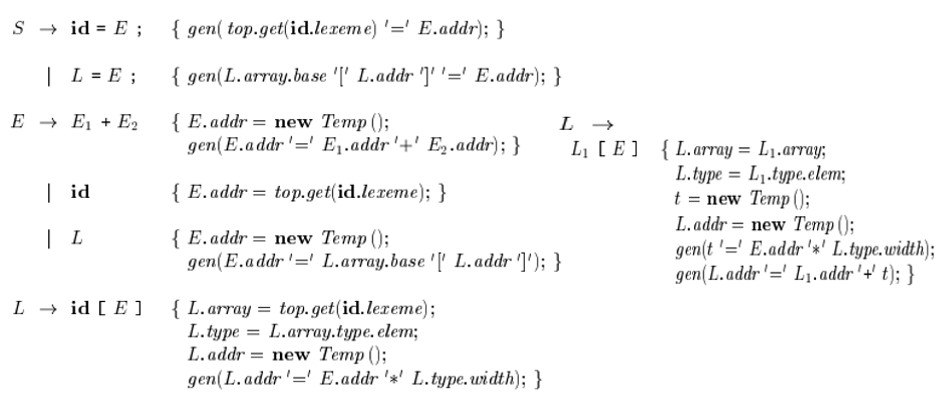
\includegraphics[width=.85\textwidth]{../../imagenes/ArrayRef}
\end{center}


\item \textbf{(2pts.)} Considera el siguiente fragmento de c\'odigo:
\begin{lstlisting}
if ( c[i] != 0 )
then 
   a[i] := b[i] / c[i];
else 
   a[i] := b[i];
\end{lstlisting}
Obtener las representaciones intermedias correspondientes a 1) \'arbol de 
sintaxis abstracta; 2) gr\'afica de control de flujo y 3) c\'odigo de tres 
direcciones. Explica tus respuestas. \\
Discutir (ampliamente) las ventajas que consideras para cada representaci\'on.

\item (Hasta 1.5pt extra). Explica lo que es una gr\'afica de control de flujo.
?`Qui\'en fue Frances Allen? 

\end{enumerate}

\end{document}
